\subsection{Architecture}
\begin{figure}
    \centering
    \subfloat[TERO loop structure \label{img:TERO_LOOP}]{
        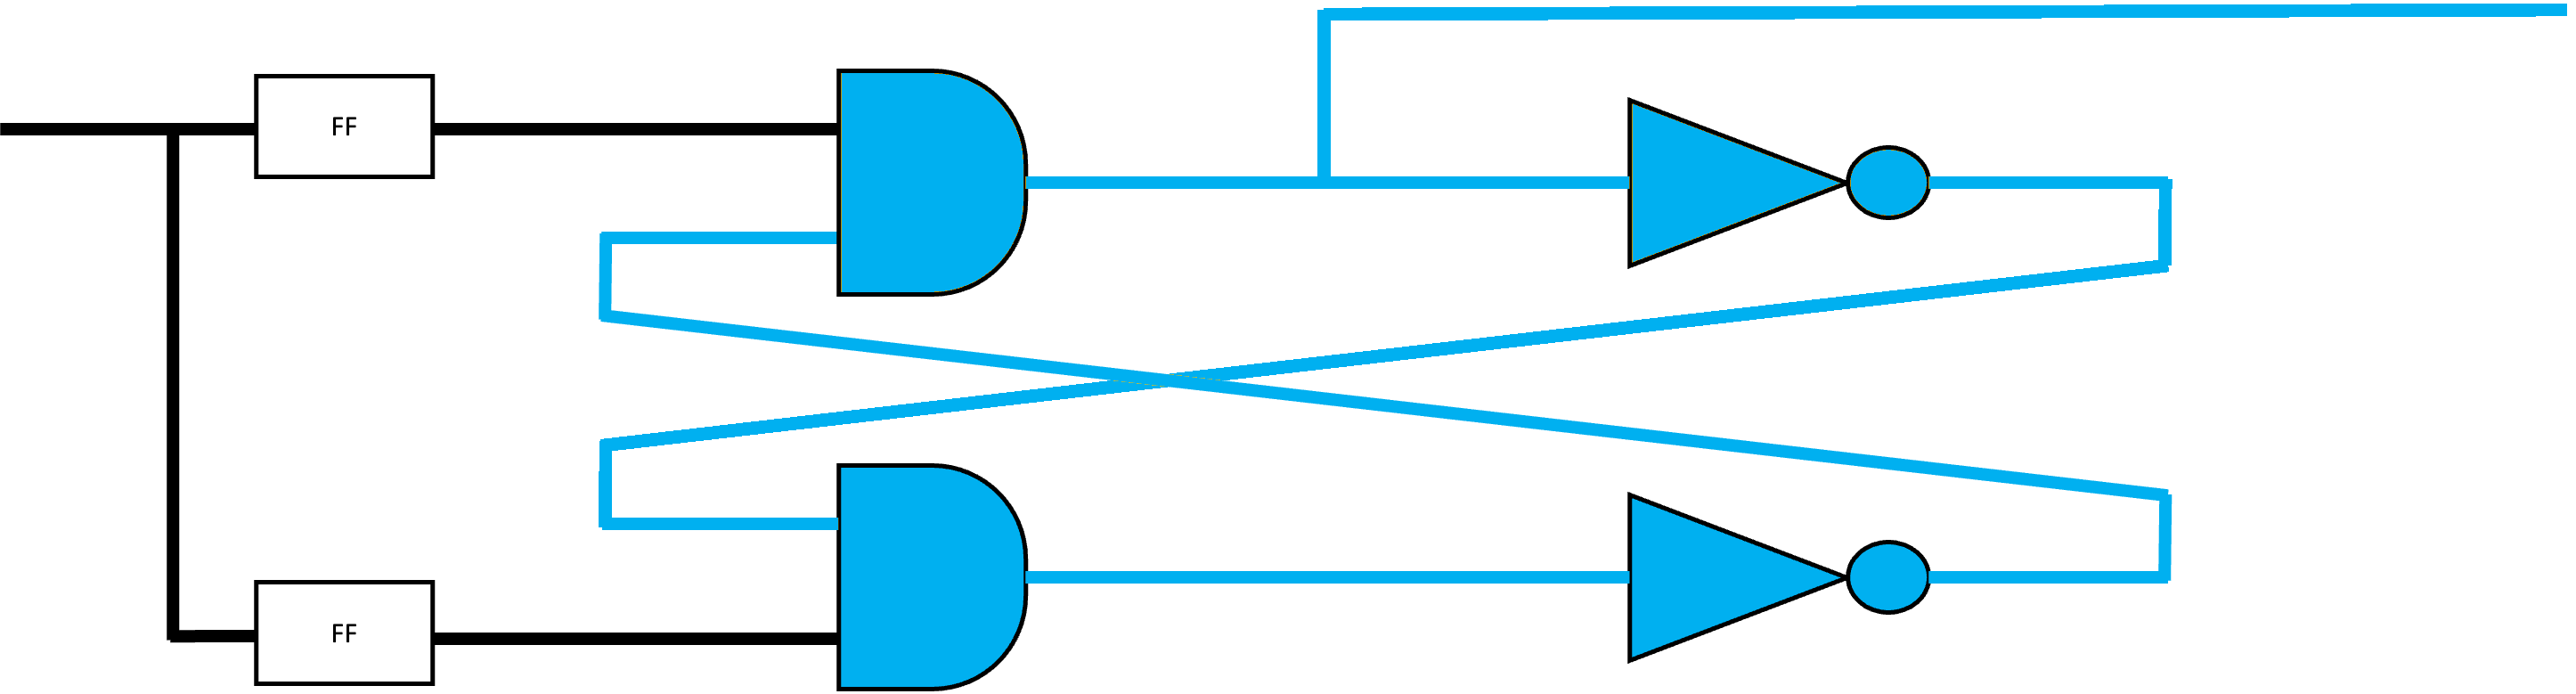
\includegraphics[scale=0.3]{TERO_loop.png}
    }
    \subfloat[2-stages counter \label{img:TERO_COUNTER}]{
        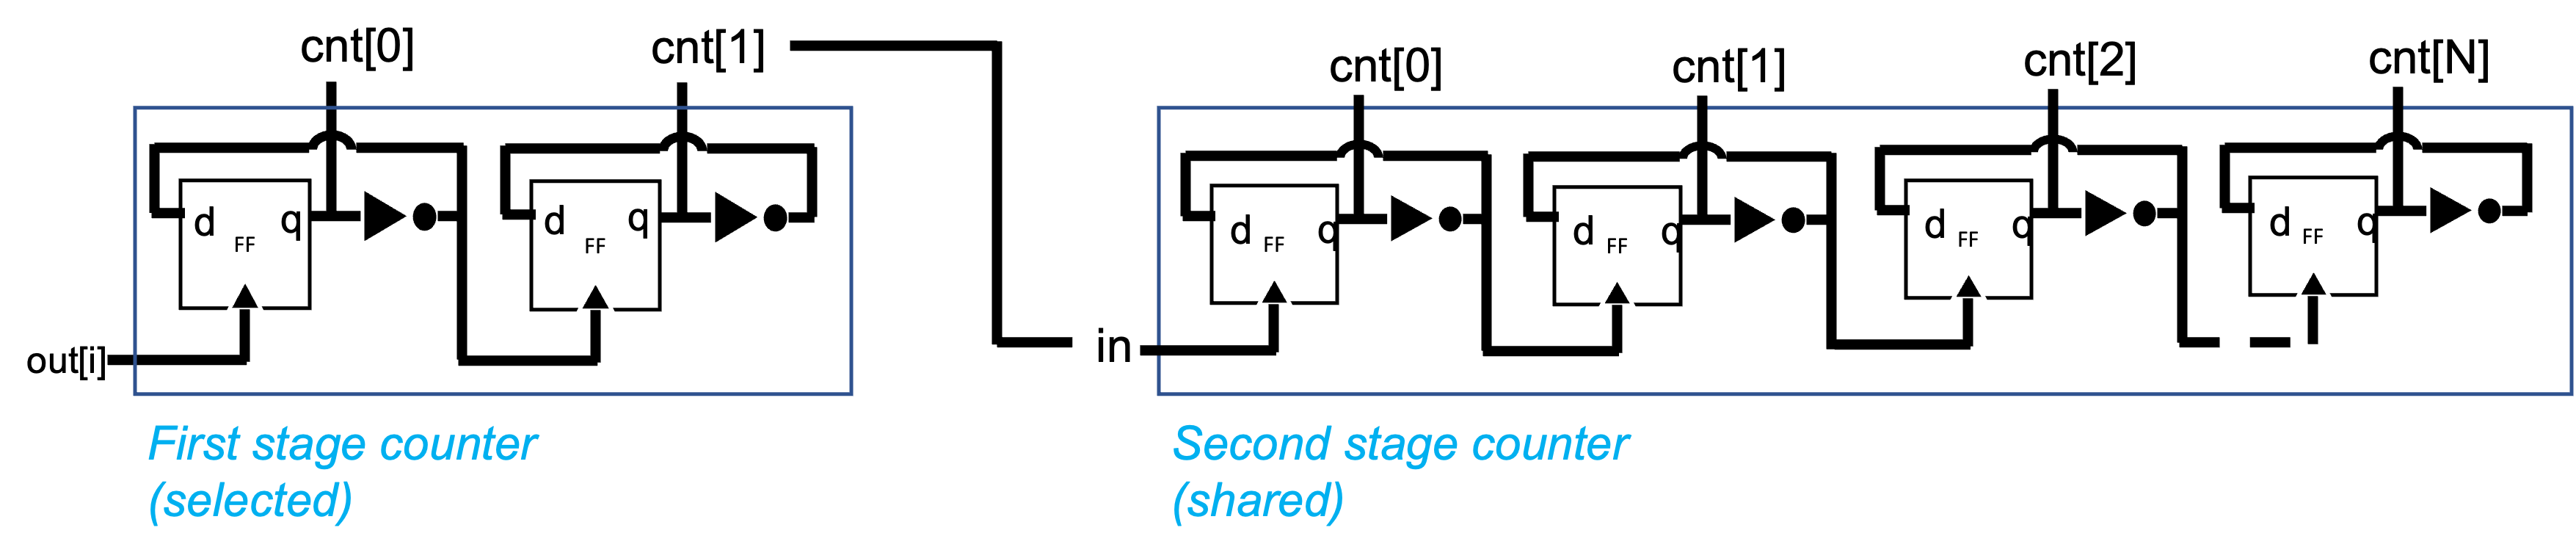
\includegraphics[scale=0.4]{TERO_counter.png}
    } 
    \caption{Structure of TERO loop and 2-stages counter}
\end{figure}
The TERO PUF is composed of a variable number of TERO loops. Each of them is based on
two AND gates and two inverters (see \textit{Figure~\ref{img:TERO_LOOP}}). \\
The two inverters are cross-coupled and brought into an unstable state via AND gates. 
While the loop tries to resolve the unstable state, it oscillates for a short time.
The number of oscillation of each loop is counted using a two-stages counter (see \textit{Figure~\ref{img:TERO_COUNTER}}).
Combining the outcomes of the loops with a specific algorithm (see \textit{Section~\ref{sec:id_generation}}),
we can obtain the overall response of the TERO PUF (ID of the FPGA). \\
In an Artix-7 Slice we can put two TERO loops (see \textit{Figure~\ref{img:TERO_CONNECTIONS}}), differing for the internal routing.
These TERO slices are arranged in four adjacent columns, placed in two different positions in the FPGA (see \textit{Figure~\ref{img:TERO_PLACEMENT}}).
\begin{figure}[h]
    \centering
    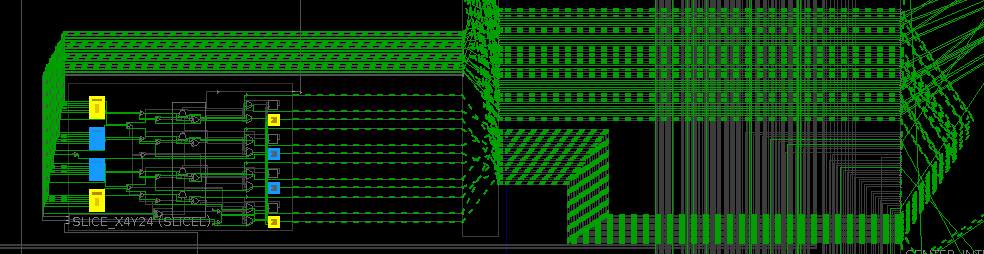
\includegraphics[scale=0.5]{TERO_connections.png}
    \caption{Connection of the two TERO loops inside one Slice}
    \label{img:TERO_CONNECTIONS}
\end{figure} \\
In this way, we obtain eight different types of loops 
(two for the differences at slice-instance, times four due to the column arrangement).
Each TERO loop has an enable signal that starts the oscillation when asserted. 
These signals are controlled by an FSM during an evaluation cycle, where each loop is activated and its oscillation measured and averaged.
The evaluation time and the number of measurement used for the average are design parameters (see \textit{Subsection~\ref{subsec:eval_and_repetitions}}).

\subsection{Communication}
The communication with a PC is handled by another FSM, which controls the UART module, 
the FIFO storing the loop responses and the challenge memory. \\
The protocol is the following:
\begin{enumerate}
    \item The PC sends a single byte request to start the interaction.
    \item The PUF replies with a single byte known identifier and waits for a challenge byte.
    \item The PC sends a challenge number encoded in a single byte.
    \item The PUF starts the evaluation of the TERO loops, as specified in details in \textit{Section~\ref{sec:results}}. 
          Each intermediate result is stored in a FIFO queue.
    \item When the evaluation is completed, the FIFO data is sent to the PC all-in-once.
    \item The communication can start again from 1.
\end{enumerate}
To handle the UART communication we exploited open-source Verilog designs found in the
net\footnote{can be found at \href{https://github.com/ben-marshall/uart}{\color{bluePoli}https://github.com/ben-marshall/uart}}, after verifying them.

\subsection{Challenges}
The challenge number sent to the PUF \textbf{could} be used to avoid the evaluation of all the loops.
The needed frequencies
\footnote{In this report we use the word \textbf{frequency} as synonym of number of oscillations performed by a TERO loop during an evaluation.}
depend on the algorithm used to generate the final response, during the post-processing on the PC. 
At the moment, we decided to expose all the frequencies in order to be able to experiment 
with various algorithms. 

\begin{figure}[H]
    \centering
    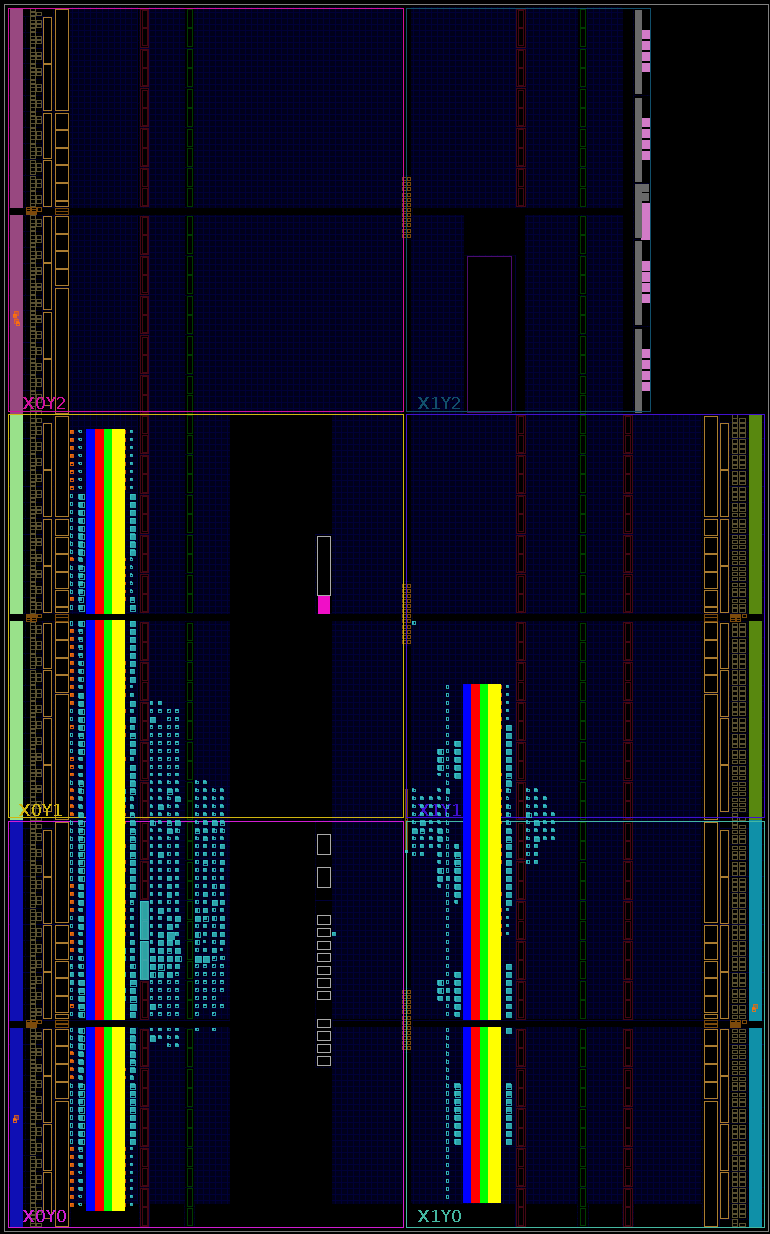
\includegraphics[scale=0.42]{TERO_placement.png}
    \caption{The TERO loops in different columns have different position in relation to the switch matrix, leading to different loop characteristics.}
    \label{img:TERO_PLACEMENT}
\end{figure}